\documentclass{article} % For LaTeX2e
\usepackage{nips13submit_e,times}
\usepackage{hyperref}
\usepackage{url}
\usepackage{amsmath}
\usepackage{bm}
\usepackage{bbm}
\usepackage{float}
\usepackage{graphicx}

\newcommand\numberthis{\addtocounter{equation}{1}\tag{\theequation}}
\DeclareMathOperator*{\argmin}{\arg\!\min}
\DeclareMathOperator*{\argmax}{\arg\!\max}

\floatstyle{boxed}
\restylefloat{figure}

\usepackage{chngcntr}
\counterwithout{figure}{section}
\counterwithout{figure}{subsection}

\title{An Optimal Control Model of Zebra Finch Vocalization}

\author{
Mike ~Schachter
\thanks{ With a metric ton of help and code from H\'{e}di Soula:
\texttt{hsoula@gmail.com}} \\
Helen Wills Neuroscience Institute\\
University of California, Berkeley\\
Berkeley, CA 94720 \\
\texttt{mike.schachter@gmail.com}
}

% The \author macro works with any number of authors. There are two commands
% used to separate the names and addresses of multiple authors: \And and \AND.
%
% Using \And between authors leaves it to \LaTeX{} to determine where to break
% the lines. Using \AND forces a linebreak at that point. So, if \LaTeX{}
% puts 3 of 4 authors names on the first line, and the last on the second
% line, try using \AND instead of \And before the third author name.

\newcommand{\fix}{\marginpar{FIX}}
\newcommand{\new}{\marginpar{NEW}}

\nipsfinalcopy % Uncomment for camera-ready version

\begin{document}

\maketitle

\begin{abstract}
In this work, a nonlinear oscillator modeling the syringeal folds of the
Zebra Finch is controlled by the state of higher level linear dynamical system.
We formulate an optimal control cost function and solution for the learning of
bird song.
\end{abstract}

\section{Introduction}

First we'll discuss the Zebra Finch vocalization system and it's mathematical
formulation, and then the control of that system. All code used to generate
figures and results in this paper can be found at:
\begin{center}
   \url{http://github.com/mschachter/birdy}
\end{center}

\subsection{The Zebra Finch Vocalization System}

Like human speech, Zebra Finch song is generated at it's source by oscillations in airflow
generated by vibrating vocal cords \cite{Mindlin2005}. Figure \ref{fig:vocal_tract} shows the Zebra Finch
synrinx.

\begin{figure}[h]
\centering
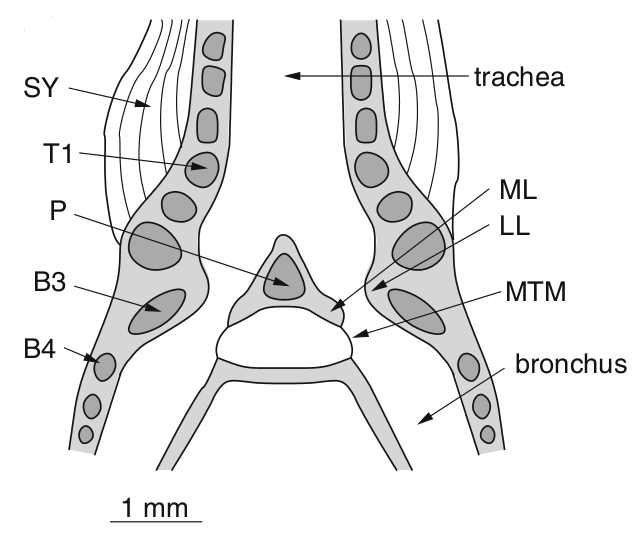
\includegraphics[width=0.5\textwidth]{images/tracheobronchial_syrinx.png}
\caption{The Zebra Finch synrinx, with two independently controlled vocal cords.}
\label{fig:vocal_tract}
\end{figure}


Each syrinx is modeled as a symmetric pair of nonlinear mass-springs. A model for
these nonlinear oscillations is taken from \cite{Sitt2010}:

\begin{align*}
\dot{x}&=\begin{aligned}v\end{aligned} \\
\dot{v}&=\begin{aligned}\gamma^2 \alpha + \gamma^2 \beta x - \gamma^2 x^3 - \gamma x^2 v + \gamma^2 x^2 - \gamma x v\end{aligned} \numberthis \label{eq_oscillator}
\end{align*}

The control parameters of the model are $\alpha$ and $\beta$. $\gamma$ = 23500 is a constant.
The control space has a rich bifurcation structure, with both Hopf and saddle-node in a
limit cycle bifurcations leading to the birth of oscillations.

\subsection{Control of the Syrinx Model}

The goal is to control the parameters $\alpha$ and $\beta$ in order to produce an observed
vocalization. Let $\bm{\phi}(t) = \left[ \alpha(t) ~ \beta(t) \right]^T$ be the state vector.

Assume that the temporal evolution of $\bm{\phi}(t)$ is defined by a controlled linear dynamical
system:

\begin{align*}
\dot{\bm{\phi}}=A\bm{\phi}(t) + \bm{u}(t)
\end{align*}

where $A$ is a 2x2 matrix, chosen to make the passive dynamics of the control system decay
to some physiologically relevant rest state.

We discretized time to simplify the analysis. Let $\Delta\tau$ be the time step for
simulation of the control system, and define $t_k = k\Delta\tau$. Also define
$\bm{\phi}_k = \bm{\phi}(t_k)$. Note that the time step for the simulation of the
control is significantly larger than that of the oscillator. In practice we used the
discrete time map representing the control system as given by the forward Euler step:

\begin{align*}
\bm{\phi}_{k+1} &= \begin{aligned}\left( A \left( \bm{\phi}_k - \bm{\phi}_{center} \right) + \bm{u}_k \right) \Delta\tau + \bm{\phi}_{k}\end{aligned} \numberthis \label{eq_control}
\end{align*}

In optimal control theory \cite{Todorov2002}, a cost function is specified and is to be minimized over time to
produce an optimal control law. But what form should the cost function take? We'll make
the following assumptions:

\begin{enumerate}

\item The control wants to keep the system's instantaneous energy low: $\bm{\phi}_k^T \bm{\phi}_k$.
\item The control wants to keep it's own instantaneous energy low: $\bm{u}^T \bm{u}$ 
%\item The control varies smoothly, i.e. $\| \bm{\phi}_k - \bm{\phi}_{k-1} \|$ is small.
\item The control wants to produce an instantaneous fundamental frequency that matches that of a stored template.

\end{enumerate}

To elaborate on the last assumption, say we are the given time-varying fundamental frequency
of a song syllable that we would like to learn, represented as the function $F(t_k)$. Let:

\begin{align*}
\hat{F} = g(\bm{\phi}_k) \numberthis \label{eq_ff}
\end{align*}

be the function that gives the steady state fundamental
frequency for a given control $\bm{\phi}_k$. The function $g$ can be empirically
estimated through simulation and approximated through interpolation. To follow this
frequency means to keep the quantity $\left( F(t_k) - g(\bm{\phi}_k) \right) ^2$ small.

Given these assumptions, the cost at time $t_k$ of applying control $\bm{u}$ is:

\begin{align*}
\ell_k \left( \bm{\phi}_{k}, \bm{u} \right) = \bm{\phi}_{k}^T \bm{\phi}_{k} +
							\bm{u}^T \bm{u} +
							%\| \bm{\phi}_{k} - \bm{\phi}_{k-1} \| +
							\left( F(t_{k+1}) - g(\bm{\phi}_{k+1}) \right) ^2
\end{align*}

Let $N$ be the number of time points we want to control, and let
$\bm{\pi}_j=\{ \bm{u}_j(\bm{\phi}_{j}), ..., \bm{u}_N(\bm{\phi}_{N}) \}$ be the control
law applied from time $j$ to time $N$. Note that the control law is a sequence of
functions! Each control uses feedback information about most recently observed state.
The total cost of applying a control law $\bm{\pi}_0$ given initial state
$\bm{\phi}_0$ is:

\begin{align*}
v\left( \bm{\phi}_0, \bm{\pi}_0 \right) = \sum_{k=1}^N \ell_k \left( \bm{\phi}_{k}, \bm{u}_k \right)
\end{align*}


\subsection{Dynamic Programming Solution to Optimal Control}

The optimal cost-to-go is a function that represents the total cost from a time
$j$ to time $N$ given that the optimal control function is applied:

\begin{align*}
v^*_j \left( \bm{\phi}_j \right) = \min_{\bm{\pi}_j} \sum_{k=j}^N \ell_k \left( \bm{\phi}_k, \bm{u}_k \right)
\end{align*}

Dynamic programming is typically used to solve for the optimal cost-to-go \cite{Bertsekas2000}. When applying
DP, we work backwards in time, creating a recursive algorithm that determines the
functional form of the entire optimal control policy $\bm{\pi}_0^*$. To illustrate
this, we are going to take $N=2$ with a specified initial condition $\bm{\phi}_0$.

First the solution must be found for $N=2$:

\begin{align*}
v^*_2 \left( \bm{\phi}_2 \right) = \min_{\bm{u}_2} \ell_2 \left( \bm{\phi}_2, \bm{u}_2 \right)
\end{align*}

A straighforward but expensive way to solve would be to perform a search over a
grid of values for $\bm{\phi}_2$. For each value on the grid, we then will use
gradient descent to minimize $\ell_2 \left( \bm{\phi}_2, \bm{u}_2 \right)$ with
respect to $\bm{u}_2$. The end result is that we have a lookup table of values,
giving us a function $\bm{u}_2(\bm{\phi}_2)$, and a function
$v^*_2 \left( \bm{\phi}_2 \right)$.

The optimal cost-to-go at time $N-1=1$ is

\begin{align*}
v^*_{1} \left( \bm{\phi}_{1} \right) = \min_{\bm{u}_{1}} \left[ \ell_1 \left( \bm{\phi}_{1}, \bm{u}_{1} \right) + v^*_2 \left( \bm{\phi}_2 \right) \right]  \numberthis \label{eq_dp} 
\end{align*}

We know the functional form of $\ell_1 \left( \bm{\phi}_{1}, \bm{u}_{1} \right)$ and the
numerical form of $v^*_2 \left( \bm{\phi}_2 \right)$. We also know that:

\begin{align*}
\bm{\phi}_2 = \left( A\bm{\phi}_1 + \bm{u}_1 \right) \Delta\tau + \bm{\phi}_1
\end{align*}

so we can again use gradient descent for a grid on $\bm{\phi}_1$ to create a lookup
table for $\bm{u}_1(\bm{\phi}_1)$ and $v^*_1 \left( \bm{\phi}_1 \right)$. We now have
a functional form for the optimal control policy: $\bm{\pi}_0^* = \{ \bm{u}_1(\bm{\phi}_1), \bm{u}_2(\bm{\phi}_2) \}$

Now going foward in time, with the knowledge of a start state $\bm{\phi}_0$, we can 
compute $\bm{\phi}_1$, and then the optimal control $\bm{u}_1 \left( \bm{\phi}_1 \right)$.
Given $\bm{u}_1$, we can then compute $\bm{\phi}_2$ and then $\bm{u}_2$. The technique
is generally applicable for any $N$.


\subsubsection{A More Efficient Implementation}
\label{section_implementation}

Solving the dynamic programming problem at a time $t_k$ requires finding a function
$\bm{u}_k(\bm{\phi}_k)$ that minimizes $v_k(\bm{\phi}_k)$ for any
$\bm{\phi}_k \in \mathcal{P}$, where $\mathcal{P}$ is a pre-specified
set of realistic values. This requires us to uniformly
sample from $\mathcal{P}$ and solve an optimization problem for each sample, a
very computationally expensive prospect!

To reduce the computational burden, we first model the function $\bm{u}_k(\bm{\phi}_k)$
as a linear combination of $M$ radial basis functions
$\{ \psi_1, ..., \psi_M \}$. Each basis function takes the form:

\begin{align*}
\psi_i(\bm{\phi}) = exp \left( \frac{\| \bm{\phi} - \bm{\theta}_i \| ^2 }{\sigma_i ^2} \right) \numberthis \label{eq_rbf} 
\end{align*}

where $\bm{\theta}_i$ is the center of the basis function, $\sigma_i$ is the bandwidth of
the basis function. Each basis function is multiplied by a coefficient
$\bm{c}_i = \left[ c_{i1} ~ c_{i2} \right]^T$. Let $\bm{C}=\left[ \bm{c}_1, ... ,\bm{c}_M \right]$
be the $2xM$ matrix of coefficients, the control is computed for a given $\bm{C}$ as:

\begin{align*}
\bm{u}_k(\bm{\phi}_k, \bm{C}) = \sum_{i=1}^M \bm{c}_i \psi_i(\bm{\phi}_k)  \numberthis \label{eq_u_rbf}
\end{align*}

We then formulate a single optimization problem to minimize the sum of cost
across all points in $\mathcal{P}$ for a given $\bm{C}$:

\begin{align*}
\bm{C}^* = \argmin_{\bm{C}} \sum_{\bm{\phi} \in \mathcal{P}} v_k( \bm{\phi}, \bm{C} )  \numberthis \label{eq_cstar}
\end{align*}

The optimal control at time $t_k$ is then given as $\bm{u}_k(\bm{\phi}_k, \bm{C}^*)$.

To create an initial guess for the optimization problem, each $\bm{c}_i$ is initialized
independently by finding the minimum cost control at $\bm{\theta}_i$, the center of
basis function $i$:
   
\begin{align*}
\bm{c}_i^0 = \argmin_{\bm{c}_i} v_k( \bm{\theta}_i, \bm{c}_i )  \numberthis \label{eq_ci}
\end{align*}


\section{Methods and Results}

\subsection{Simulation}

Equation \eqref{eq_oscillator} was implemented in C++ and utilized the GNU Scientific Library. It
was accessed and simulated using Cython/Python. The integration method used was an 8th order
Runga-Kutta method \cite{JRDormand1980} with a step size of 1 $\mu s$. A GUI was created using
PyQT in order to examine the dependence of oscillations with the control parameters, as
shown in figure \ref{fig:simulation}.

\begin{figure}[h]
\centering
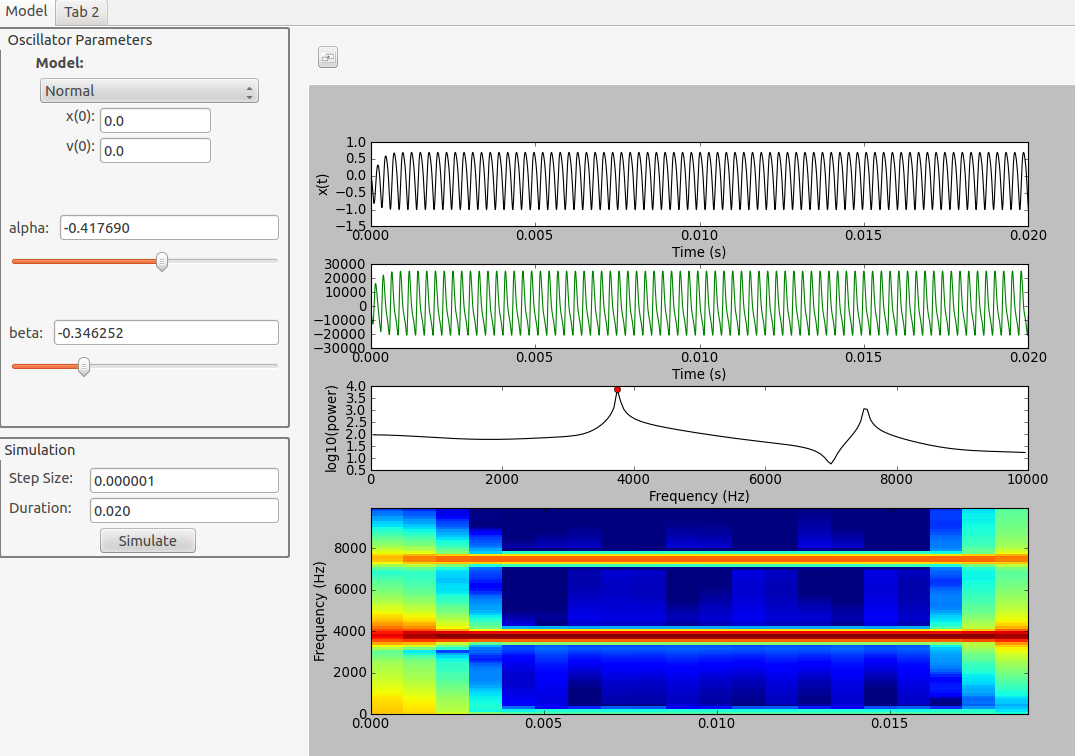
\includegraphics[width=0.75\textwidth]{images/simulation.png}
\caption{The UI for the simulation environment.}
\label{fig:simulation}
\end{figure}

\subsection{Mapping Controls to Fundamental Frequency}

Equation \eqref{eq_ff} maps a control $\bm{\phi}$ to a steady-state fundamental frequency
$\hat{F}$, and required simulation to determine. First, a grid of points was constructed that spanned
$\alpha \in [-1.25, 0.05]$ and $\beta \in [-1.10, 1.10]$, with a spacing of 0.05. For each
point in the grid, the oscillator was simulated with a zero initial condition and the control
specified by the grid point, for 15 ms.

The power spectrum of the resluting oscillation was
taken and the fundamental frequency $\hat{F}$ was identified as it's maximum. This
produced samples for a real-valued function of two variables. These samples were fit with
a radial basis function implementation from SciPy with a bandwidth 0.8 and Gaussian kernel.
A RBF kernel was placed at each of the sample points, and allowed for a continuously-varying
representation of equation \eqref{eq_ff}. The sampling and it's RBF interpolation are shown
in figure \ref{fig:ff}.

\begin{figure}[h]
\centering
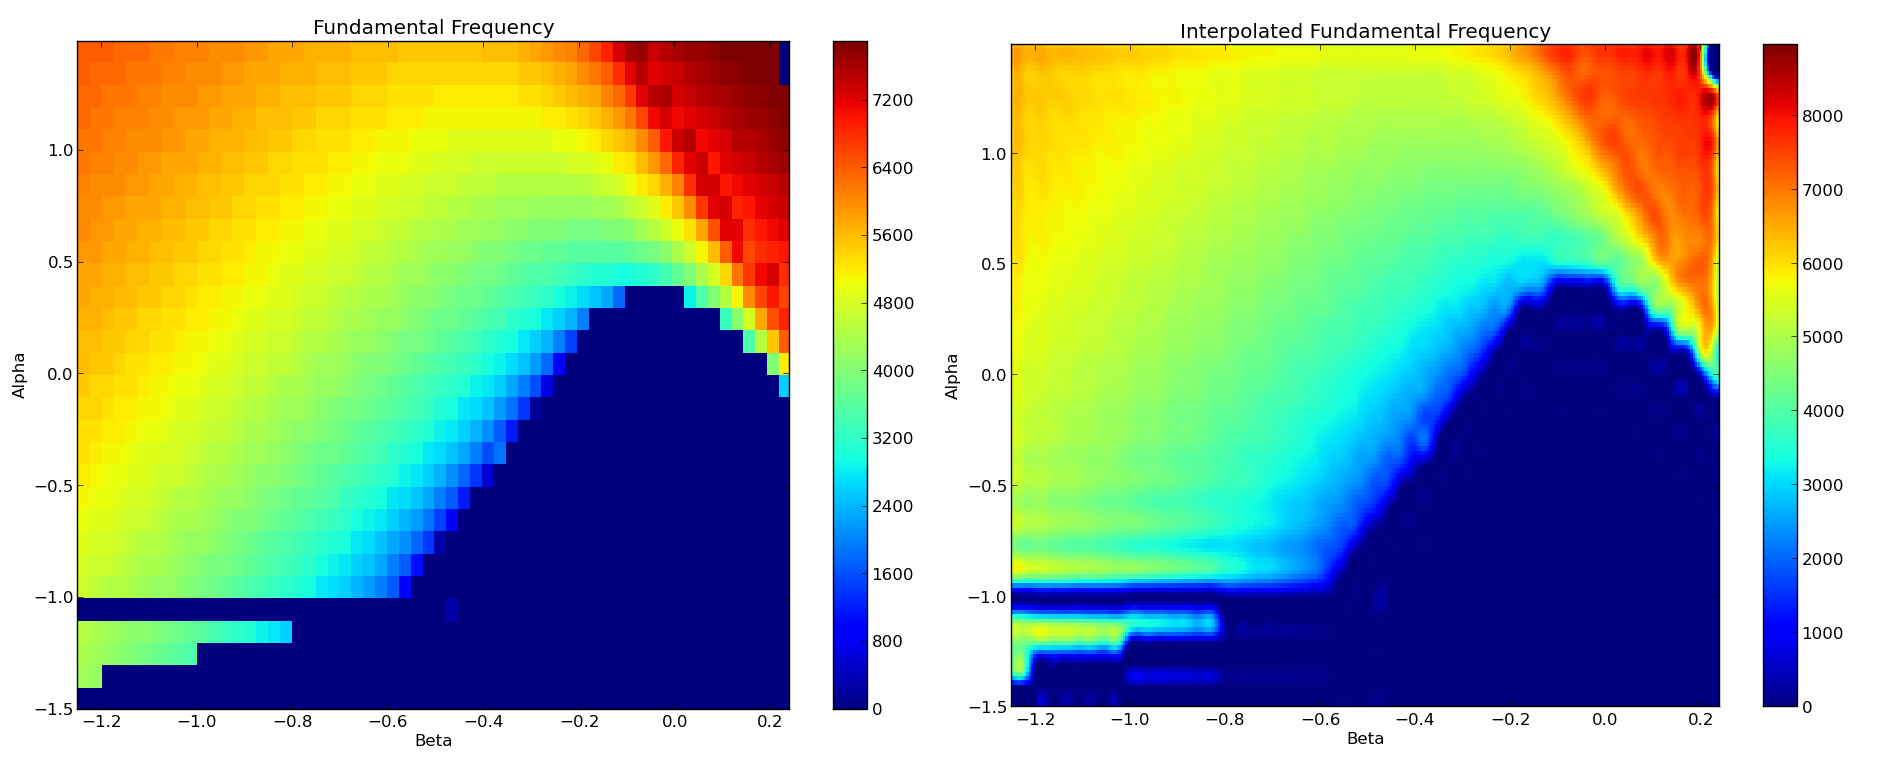
\includegraphics[width=1.0\textwidth]{images/ff_both.png}
\caption{The simulated steady-state fundamental frequency as a function of control (left), and it's interpolation by radial basis functions (right).}
\label{fig:ff}
\end{figure}

\subsection{Optimal Control}

The first step in solving the optimal control problem was to choose the passive dynamics
of the system defined by \eqref{eq_control}. We chose the following matrix:

\begin{align*}
A = \left[ \begin{array}{cc} -1000 & 0 \\ 0 & -900 \end{array} \right]
\end{align*}

and specified $\bm{\phi}_{center} = \left[ -0.30 ~ 0.30 \right] ^T$. The passive
dynamics had the phase plot specified in figure \ref{fig:phase_plot}. The values
of $A$ were specified such that both $\alpha$ and $\beta$ decayed to their rest
points within 10ms.

\begin{figure}[h]
\centering
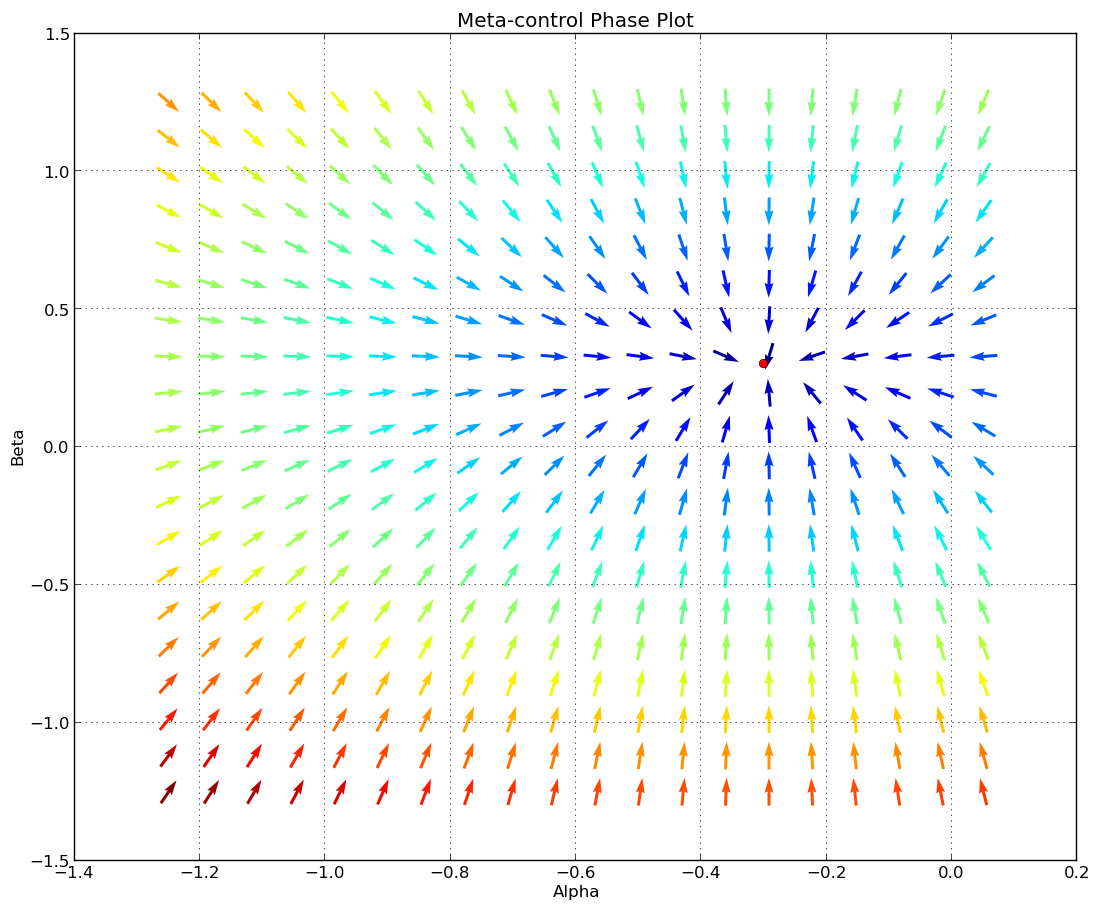
\includegraphics[width=0.75\textwidth]{images/passive_phase_plot.png}
\caption{A phase plot for the passive dynamics of the control system. Color indicates magnitude, red is large, blue is small.}
\label{fig:phase_plot}
\end{figure}

Once the passive dynamics were selected, we applied the algorithm described in section
\ref{section_implementation}. First, we created a grid of points for $\bm{u}$ that
spanned $[-1,1] X [-1, 1] \subset \mathbbm{R}^2$, with a spacing of 0.25. Each point
in the grid was a center $\bm{\theta}_i$ as listed in equation \eqref{eq_rbf}. The bandwidths
were chosen uniformly as $\sigma_i = 0.30$.

In the next step, the desired sequence of fundamental frequencies was specified with
a sample spacing of $1ms$. The last frequency in the sequence was selected, and the
dynamic programming optimization began.

The goal of the DP algorithm, for a given time step, was to determine the matrix
$\bm{C}^*$ of equation \eqref{eq_cstar}. $\bm{C}^*$ was then used in equation 
\eqref{eq_u_rbf} to determine the optimal control.

Because the optimization problem of \eqref{eq_cstar} is (probably) difficult and
(possibly) nonconvex, and definitely expensive, the first step was to find a good
initial guess for each element of $\bm{C}^*$. So we evaluated a locally-optimal
value at each center, solving the optimization problem specified by equation
\eqref{eq_ci}. This was accomplished using gradient descent, with an initial
guess of $\bm{c}_i^0 = \left[ 0 ~ 0 \right] ^T$. All gradients were computed using
a finite-difference approximation.

Once $\bm{C}$ was initialized, we then ran the full optimization of equation
\eqref{eq_cstar}. We only let it run for 10 iterations, with the intention of
actually getting at least one result before the due date of this project!

The technique above was applied to the last time point. Using dynamic programming,
we then solved for the second-to-last time point, applying a recursion to the cost
similar to that shown in equation \eqref{eq_dp}. The time for optimization increased
linearly as a function of how far back in time we went, as shown in figure \ref{fig:optimization_time}.

\begin{figure}[h]
\centering
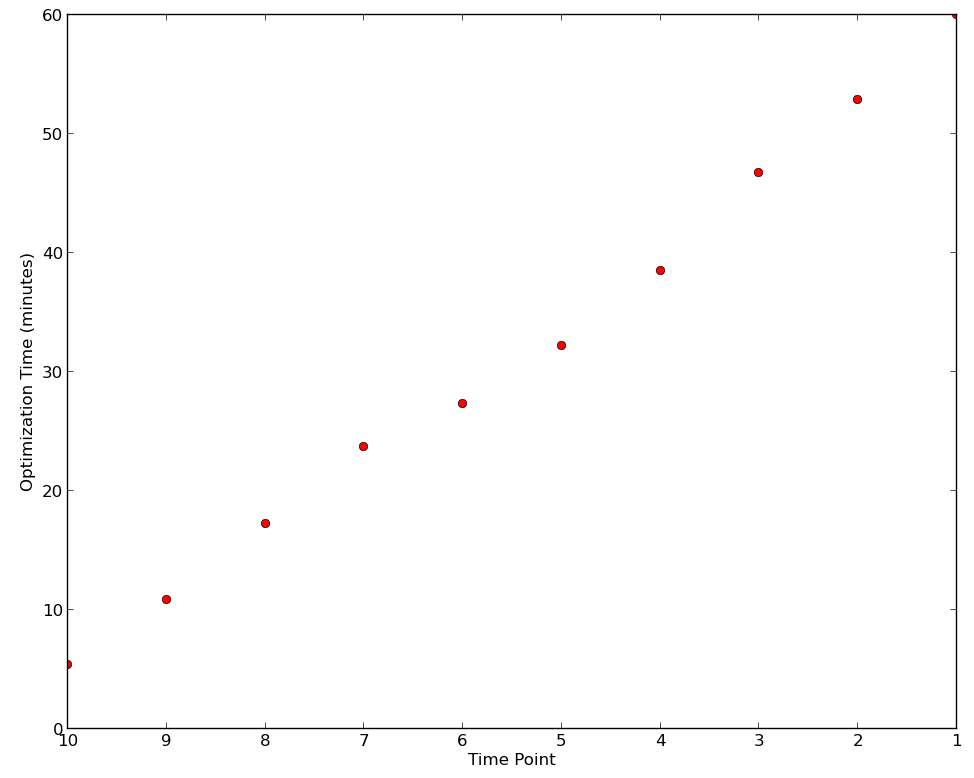
\includegraphics[width=0.5\textwidth]{images/optimization_time.png}
\caption{The computation time for optimization at each time point.}
\label{fig:optimization_time}
\end{figure}

Given time constraints, we only had the opportunity to apply the equation to a single
example, that of a constant desired fundamental frequency of 3000Hz for 10ms. The total
time to solve this problem, computed as the cumulative sum of the times in figure
\ref{fig:optimization_time}, was 314 minutes.

For each time point, we determined the form of the function specified in \eqref{eq_u_rbf}. One
such example of this function is shown in figure \ref{fig:cost_and_control}. Some explanation
is in order. The upper left is the optimal cost-to-go function $v_{10}^*(\bm{\phi})$. It
shows that the most expensive states are those that produce a mismatch of the fundamental
frequency (see figure \ref{fig:ff}).

\begin{figure}[h]
\centering
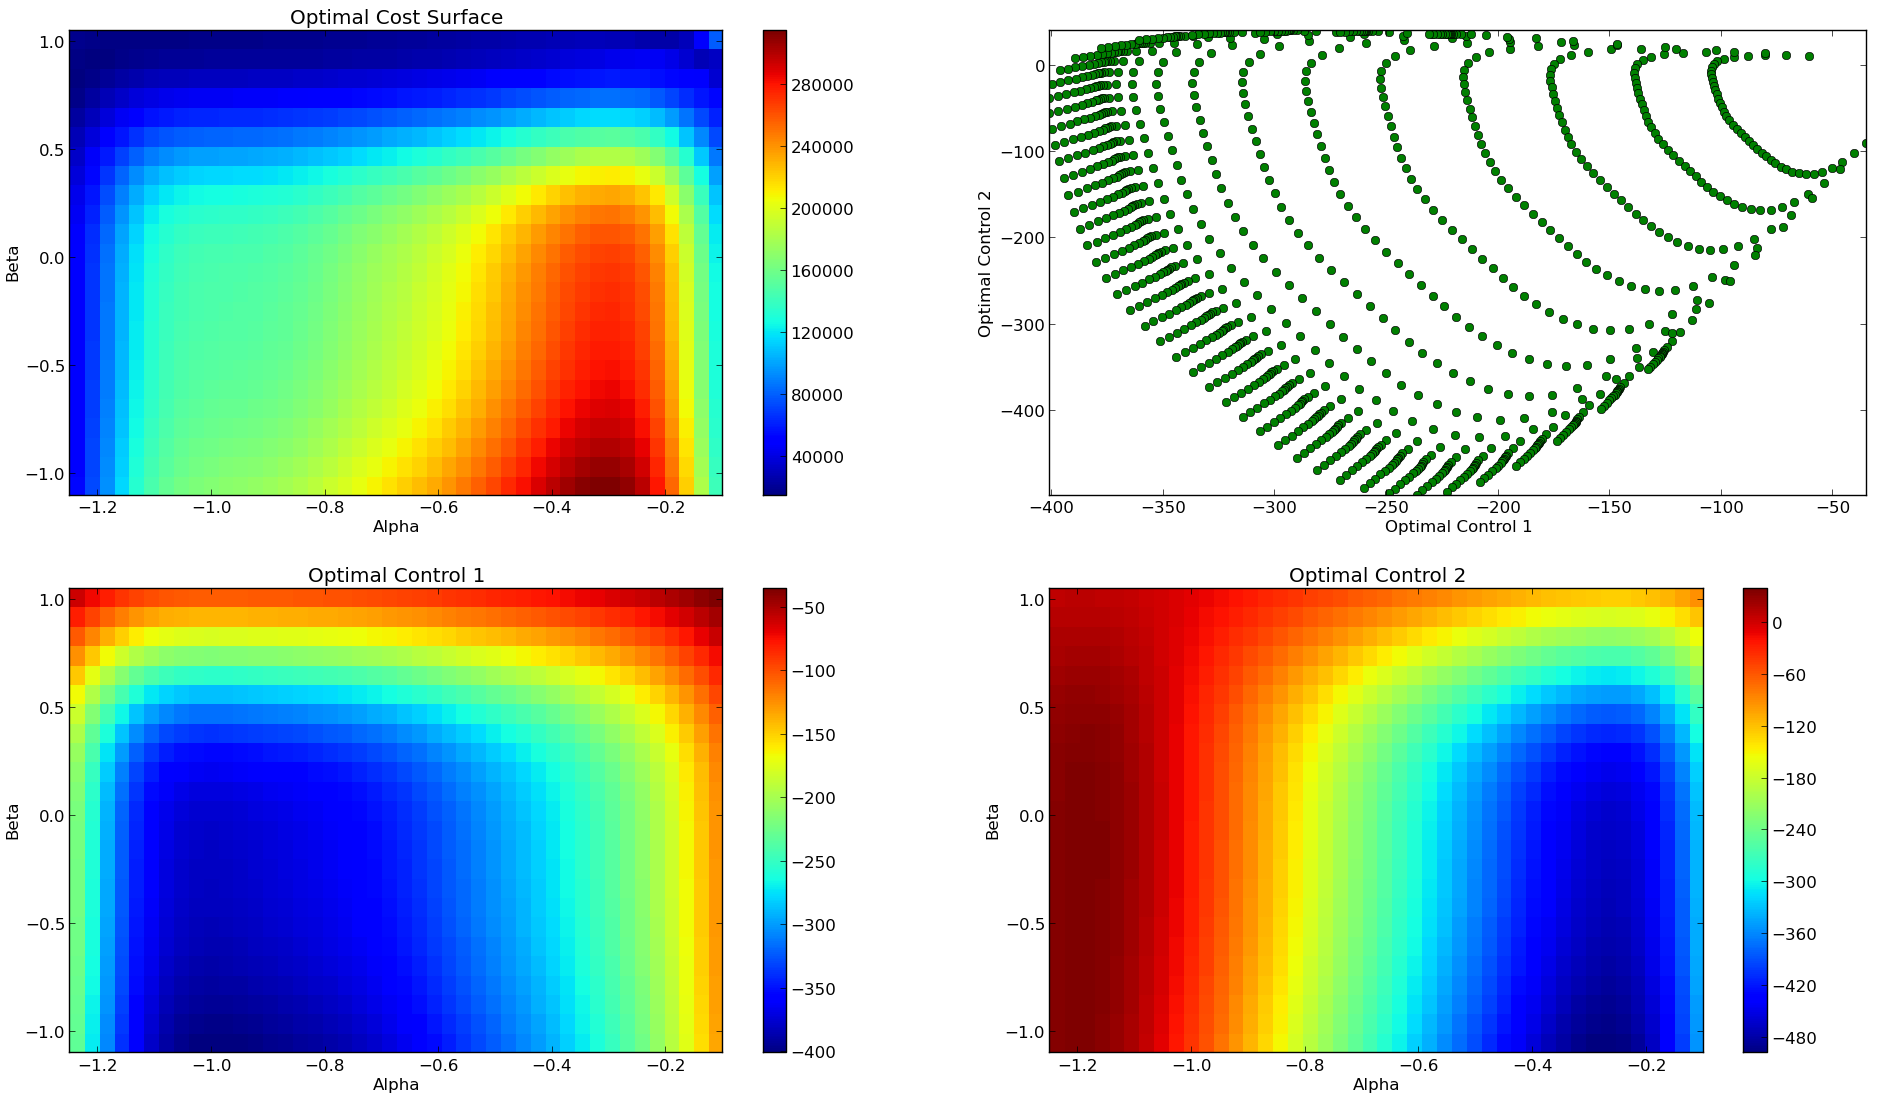
\includegraphics[width=1.0\textwidth]{images/cost_and_control.png}
\caption{Upper Left: the optimal cost-to-go function at time point $N=10$.
         Upper Right: the optimal control vector elements plotted against eachother.
         Lower Left: optimal control 1 as a function of $\bm{\phi}$.
         Lower Right:optimal control 1 as a function of $\bm{\phi}$. }
\label{fig:cost_and_control}
\end{figure}

The lower left panel shows the value of $u_0$ for a given
value of $\bm{\phi}$. Strongly negative values of $u_0$ will push $\alpha$ to be significantly
more negative. The control at this time point seems to have the ability to push $\alpha$ to
two different regions of the space, to the extreme left and to the extreme right. Given
that time has run out to check for bugs, we can only hope that this makes sense...

The lower right panel shows a tendency for the control $u_1$ to push $\beta$ into a negative
range, dependent on the value of $\alpha$. It's probably best not to over-interpret this
figure in the absence of a more rigorous analysis of bugs. The upper right panel shows
$u_0$ vs $u_1$, showing a very much nonlinear relationship between the two.

You may ask yourself at this point, "does it work"? The answer for now is "perhaps". Figure
\ref{fig:spectrogram} is a spectrogram of a 10ms simulation for the optimal control law
applied to a given initial condition. There's plenty of power in the 3000Hz range, but again,
it's really unclear if this was just dumb-luck. More debugging is necessary!

\begin{figure}[h]
\centering
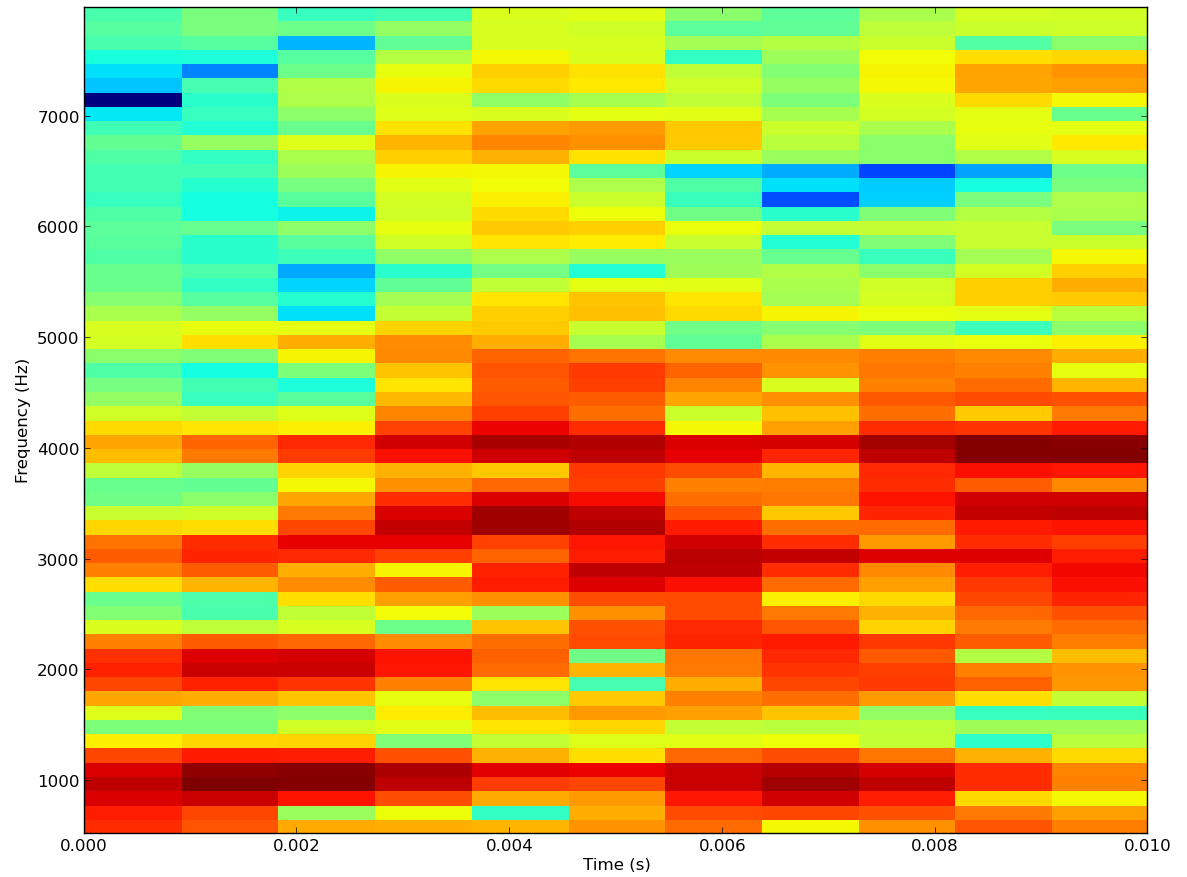
\includegraphics[width=0.75\textwidth]{images/spectrogram.png}
\caption{A spectrogram for an optimally-controlled vocalization.}
\label{fig:spectrogram}
\end{figure}


\section{Conclusion}

This work was an exciting foray into the world of nonlinear oscillators and optimal control
theory. It's a work-in-progress, setting the stage for my thesis work, which will require
the generation of synthetic Zebra Finch syllables.


\iffalse
\subsection{Temporal Hierarchy of Representation}

Generically, we want to determine a joint probability between $\bm{\phi}$ and a set of
variables that are related to the acoustic representation. These features may span several
time scales. For example, instead of just relating $F(t)$ and $\bm{\phi}$, i.e. looking
at the joint distribution $p \left( F(t), \bm{\phi} \right)$, we might want to look
at the running variance of $F(t)$ for a specified time window.

Let $\{ \sigma_1, ..., \sigma_m \}$ be a set of statistics for some acoustic variables. Construct
this set so that they are ordered by time scale. By this, we mean that computing $\sigma_i$
requires a larger window of time than computing $\sigma_j$ if $i < j$.

Finding the optimal control requires maximizing a conditional probability:

\begin{align*}
\argmin_{\bm{u}} C_f = \argmax_{\bm{\phi}(\bm{u})} p \left( \bm{\phi}(\bm{u}) | \sigma_1, ..., \sigma_m \right)
\end{align*}

There may be a "telescoping" algorithm to maximizing $p \left( \bm{\phi}(\bm{u}) | \sigma_1, ..., \sigma_m \right)$
quickly. Start with $\sigma_1$, which is the statistic with the longest time scale.
There should be many instantaneous values of $\bm{u}(t)$ that give a nonzero
probability of occurance with $\sigma_1$. But not all the values will, so restrict the
search for all $\bm{u}$ to that space. Do the same for $\sigma_2$, which will
reduce the size of the space even further. Continue this process until the space of
actual $\bm{u}$ is small enough to do a more efficient optimization, and then
peform that optimization to find the optimal control.
\fi


\section*{Acknowledgments}

Thank you to H\'{e}di Soula, who created a C++/Python implementation of this model in our lab
and has provided ideas, expertise, and feedback on this project. Extra thanks to Jim Crutchfield,
who facilitated an excellent NCASO course and offered lots of advice on this project.

\bibliographystyle{acm}
\bibliography{papers}

\end{document}

